Antes de comenzar el desarrollo vamos a definir algunos términos.

$\bullet$ \textbf{Informacion}: Dado un evento E decimos que cuando E tiene lugar, recibimos
\begin{center}
$I (E) = log(\frac{1}{P(E)})$ 
\end{center}

unidades de información. Al usar $log_2$ la unidad obtenida es bits.

$\bullet$ \textbf{Entropía}: La entropía de un mensaje X, que se representa por H(X), es el valor medio ponderado de la cantidad de información de los diversos estados del mensaje 

\begin{center}
$H(X) = - \Sigma$ $p(x)$ $log$ $p(x)$
\end{center}

$\bullet$ \textbf{Nodo distinguido}: En una fuente, un nodo distinguido es un nodo cuya información es menor a la entropía de dicha fuente.

\subsection{Capturando tráfico}
Para el desarrollo de este trabajo práctico escuchamos pasivamente redes para poder observar que sucedía en las mismas. En particular, capturamos paquetes ARP \emph{who-has}.

Utilizamos dos modelos de fuente de información:

$S_{dst}$ = \{$s_1$ $\cdots$ $s_n$\} siendo $s_i$ una IP que aparece como dirección destino en los paquetes ARP \emph{who-has}

$S_{src}$ = \{$s_1$ $\cdots$ $s_n$\} siendo $s_i$ una IP que aparece como dirección origen en los paquetes ARP \emph{who-has}

Creamos una \emph{tool} que escucha pasivamente en la red local. Luego, la adaptamos para que estime las probabilidades de dichas fuentes en función de los paquetes ARP observados y que calcule la entropía de las mismas.

Usando dicha herramienta, realizamos capturas de paquetes ARP sobre distintas LANs: Alto Palermo, Red laboral de Honeywell, Laboratorios de Ciudad Universitaria (Via Wi-Fi), y la casa de un integrante del grupo.

\subsection{Gráficos}

Una vez que capturamos el tráfico, nos propusimos gráficar y a analizar los datos obtenidos. Realizamos tres tipos de gráficos:

$\bullet$ Grafos dirigidos:
  En los grafos, los nodos son los IPs que aparecen en alguno de los paquetes capturados.
  Una arista entre A y B significa que se encontro un paquete con \emph{src} A y \emph{dst} B. El peso de cada arista corresponde a la cantidad de paquetes de la forma anterior.
  
  Ejemplo:
  
  \begin{figure}[H]
  \begin{center}
    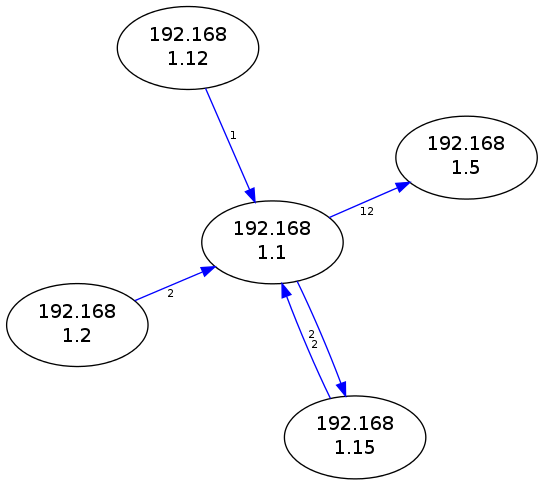
\includegraphics[width=\linewidth/2]{../imgs/red-hogarena_red.png}
    \label{fig:FedeGrafo}
    \caption{Grafo de LAN hogareña}
  \end{center}
\end{figure}

$\bullet$ Histograma:
  Realizamos para cada una de las fuentes (\emph{src} y \emph{dst}), realizamos un histograma que muestra la cantidad de apariciones de un determinado IP en la fuente.
  
  Ejemplo:
  
  \begin{figure}[H]
  \begin{center}
    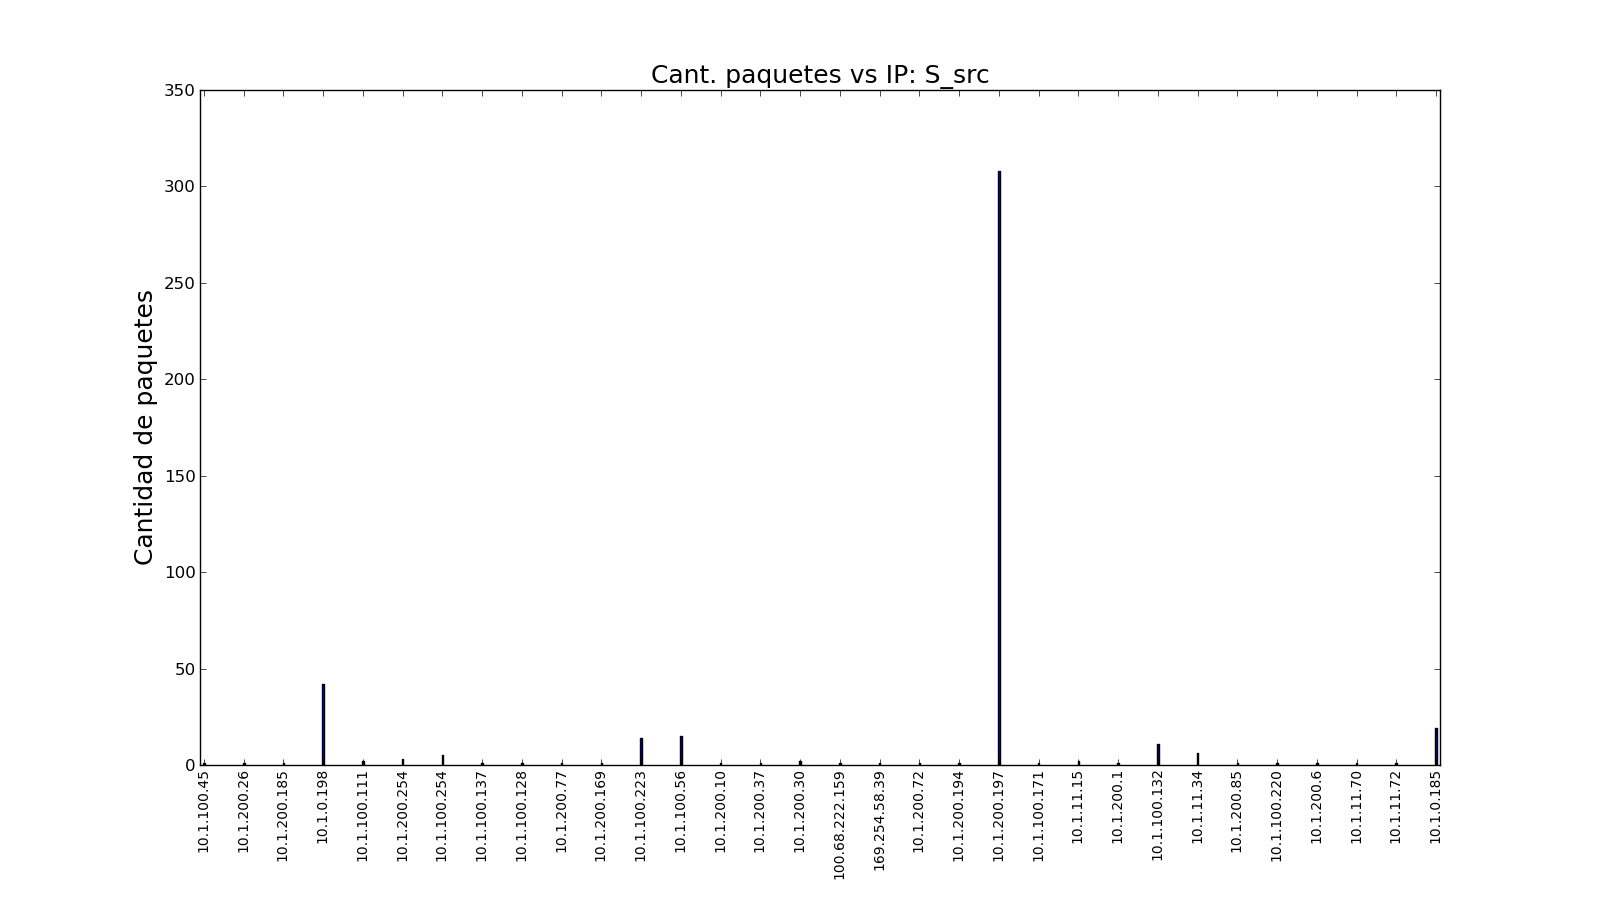
\includegraphics[width=\linewidth/2]{../imgs/red-entrepiso-dc_S_src_hist.png}
    \caption{Histograma de la serie de paquetes s\_src de la red \emph{Entrepiso-DC}.}
    \label{fig:histograma-entrepiso-dc-s-src}
  \end{center}
  \end{figure}
  
$\bullet$ Gráfico Información:
  Realizamos para cada una de las fuentes (\emph{src} y \emph{dst}), realizamos un gráfico donde se muestra la información de un determinado IP en la fuente. Además graficamos una recta con el valor de la entropía para comparar facilmente la información de cada IP con la entropía de la fuente. 
  
  Ejemplo:
  
  \begin{figure}  
  \begin{center}
    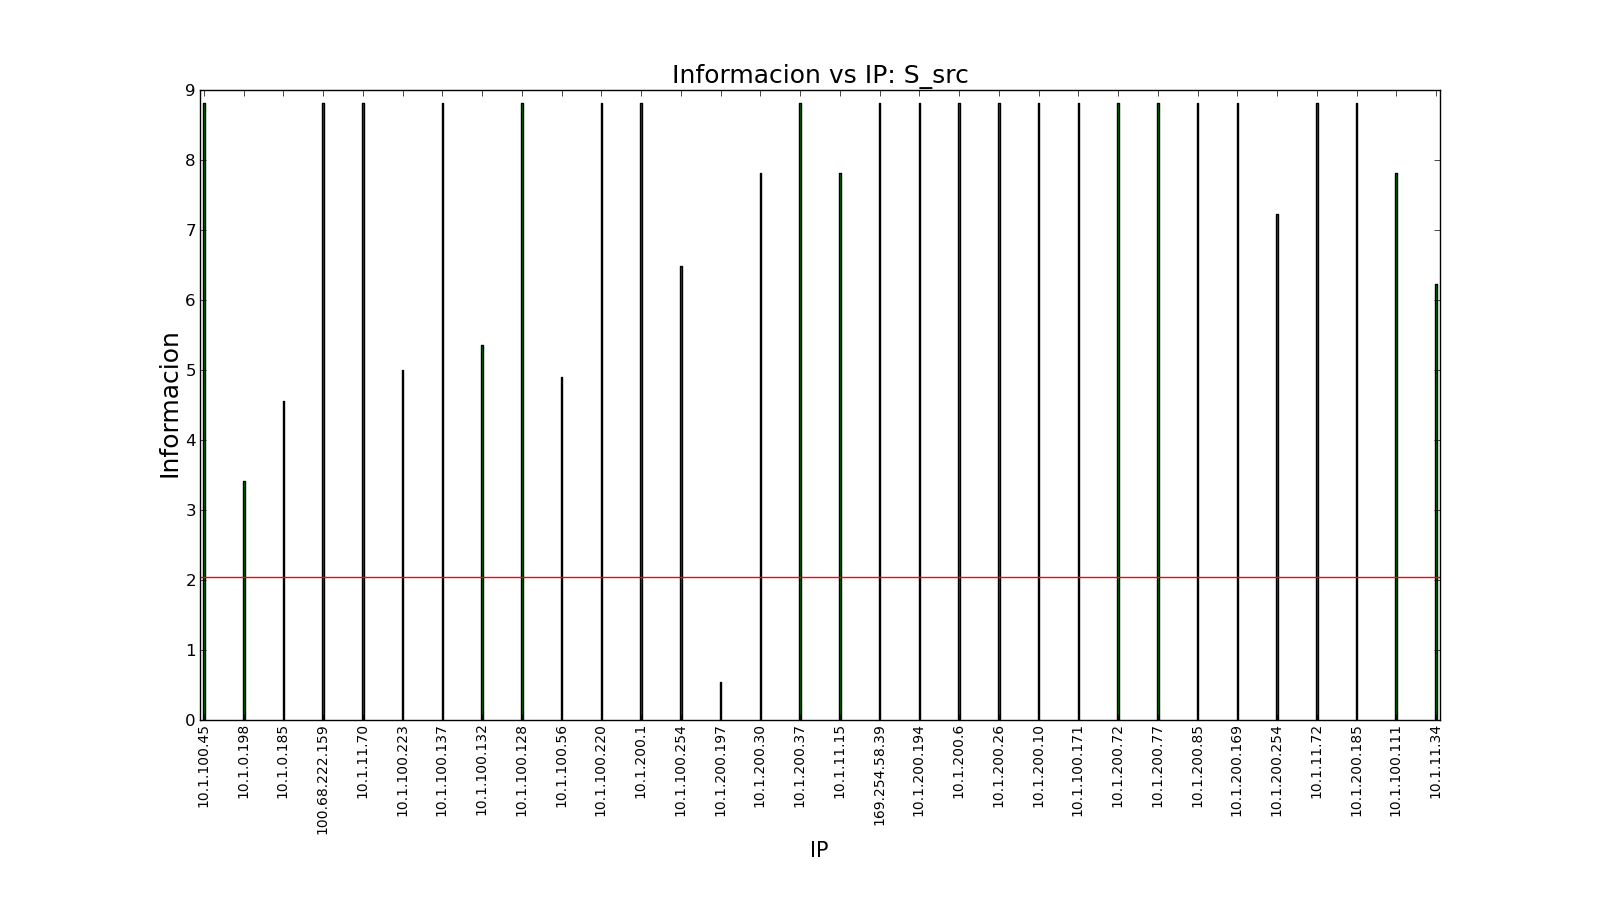
\includegraphics[width=\linewidth/2]{../imgs/red-entrepiso-dc_S_src_info.png}
    \caption{Gráfico de cantidad de información para cada IP s\_src de la red \emph{Entrepiso-DC}.}
    \label{fig:informacion-entrepiso-dc-s-src}
  \end{center}
\end{figure}
  
Graficamos en forma de histogramas, y de grafos la información y entropía de $S_{dst}$ y $S_{src}$